\documentclass[12pt]{article}
\usepackage[english]{babel}
\usepackage[utf8]{inputenc}
\usepackage{amsmath}
\usepackage{graphicx}
\graphicspath{{Images/}}
\usepackage[colorinlistoftodos]{todonotes}
\usepackage{hyperref}
\usepackage{apple_emoji}
%\usepackage{fancyhdr}
%\pagestyle{fancy}
\begin{document}
\begin{titlepage}
\newcommand{\HRule}{\rule{\linewidth}{0.1mm}} 
\center % Center everything on the page
 
%---------------------------------------------------------------------------------
%	HEADING SECTIONS (Enter the Homework/assignment No., only)
%---------------------------------------------------------------------------------
\textsc{\Large MIDDLEWARE}\\[0.5cm] % heading course Number
\textsc{\Large Design et Autonomisation d'un kart }\\[0.5cm] % heading course name
\textsc{\large Projet }\\[0.5cm] % Minor heading
%---------------------------------------------------------------------------------
%	TITLE SECTION (Replace 'TITLE' with the Homework/assignment Name/title)
%---------------------------------------------------------------------------------

\HRule \\[0.4cm]
{ \huge \bfseries KART}\\[0.1cm] % Title of your Homework/assignment
\HRule \\[1.5cm]
 
%---------------------------------------------------------------------------------
%	AUTHOR SECTION (EDIT THE NAME and T.NO., only)
%---------------------------------------------------------------------------------

\begin{minipage}{0.4\textwidth}
\begin{flushleft} \large
Gwendal \textsc{Priser}\\  % Enter Your name and T.No.
\end{flushleft}

\begin{flushleft} \large
    Paul-Antoine \textsc{Le Tolguenec}\\  % Enter Your name and T.No.
    \end{flushleft}
    \begin{flushleft} \large
        Mamadou \textsc{Dembele}\\  % Enter Your name and T.No.
        \end{flushleft}
\end{minipage}
\begin{minipage}{0.4\textwidth}
    \begin{flushleft} \large
        Quentin \textsc{Brateau}\\  % Enter Your name and T.No.
        \end{flushleft}

        \begin{flushleft} \large
            Jules \textsc{Berhault}\\  % Enter Your name and T.No.
            \end{flushleft}
\end{minipage}\\[1cm]
{\large \today}\\[1cm] % Date, change the \today to a set date if you want to be precise

\includegraphics{ENSTA1246-524.png}% \\[0.5cm] % 
\vfill % Fill the rest of the page with white-space

\end{titlepage}
\include{GradingRubric}
\tableofcontents          % Required
\listoffigures
\listoftables
\newpage

% Do not edit the below sections, enter all details in respective chapters
% Add the images/screen-shorts to the image folder and insert them in the respective chapters


\section{Introduction}
\paragraph{}In the middleware module of UV 4.1, we are asked to implement the ROS middleware to drive a small car built in the previous semester. 
This small project consists in driving around an athletics track in an autonomous way. 
To carry out this project we have various sensors such as the Inertielle control unit which estimates the heading of the car and its acceleration, the camera, 
the gps which will allow us to estimate the position of the small car. We also have an on-board computer, in this case a raspberry.

\textbf{Repo GitHub}

\url{https://github.com/gwendalp/kart}



\section{Hardware}
\sesction{Hardware}

\subsection{Introduction}

\subsection{Main Board}
\paragraph{}For this project, we decided to use a \textit{Raspberry Pi 3B+}
as main board. It will let us plug some sensors and control the motors of
the car according to the wanted behavior we have programmed.

\paragraph{}On this Raspberry Pi, we need to choose an Operating System. our
choice was to use Ubuntu Mate because of its simplicity to install and its 
polyvalence. It will let us do everything we want, like plug sensors, code
any program to control our car, ... A preview of Ubuntu Mate is shown on
the ~\ref{fig:ubuntu}

\begin{figure}[!ht]
    \begin{center}
        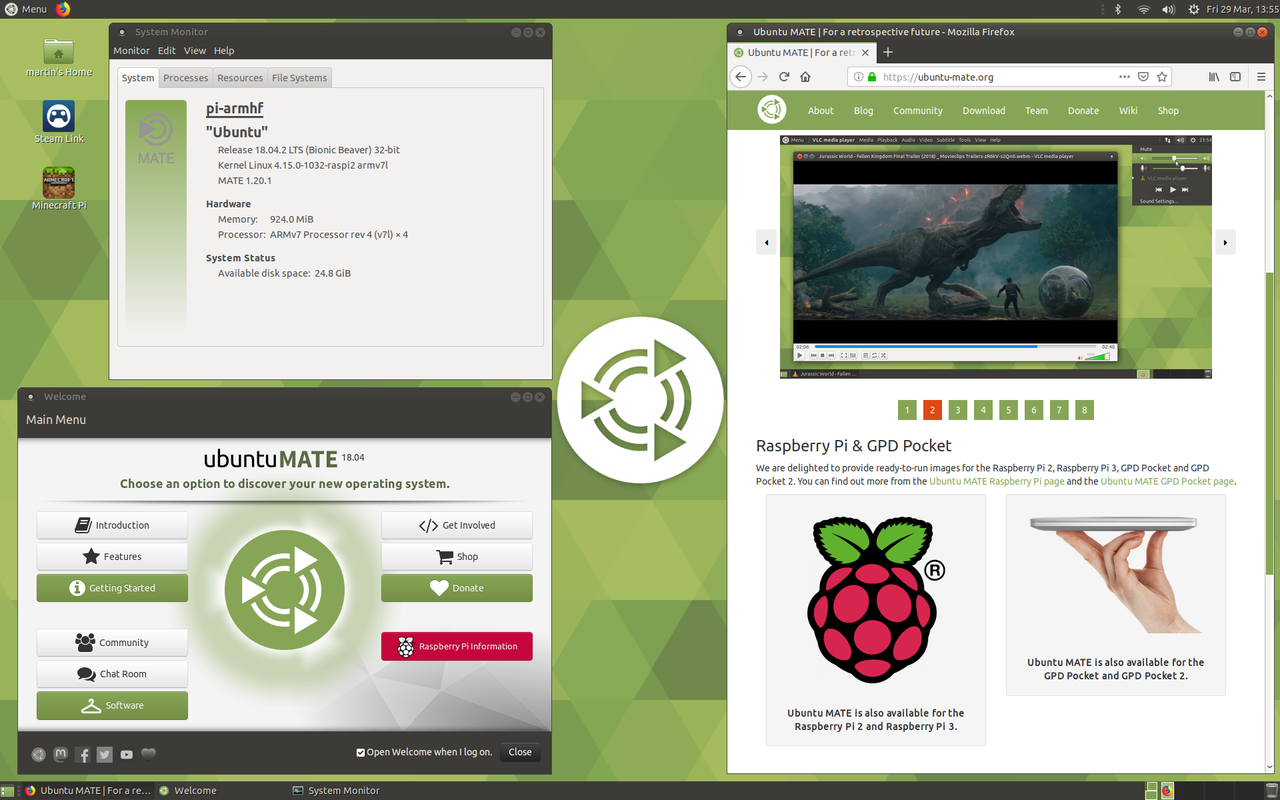
\includegraphics[scale=0.3]{Images/Ubuntu_mate.png}
    \end{center}
    \caption{Ubuntu Mate screen}
    \label{fig:ubuntu}
\end{figure}

\paragraph{}As an imposed figure for our project, we decided to use the 
\textit{Robot Operating System} (ROS) as Middleware for this car. It's
going to offer us some practical tools to code our pragrams easily.
There is also some usefull community shared tools like \textit{rqt}
or \textit{key\_telop} we will use in this project. Then we decided to
setup a graph node and to code these node in order to build our system
as shown on the following graph node.

\begin{figure}[!ht]
    \begin{center}
        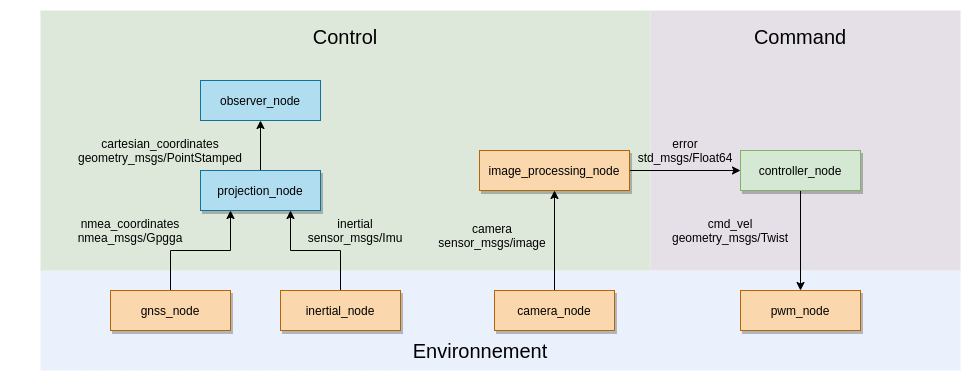
\includegraphics[scale=0.4]{Images/node_graph.png}
    \end{center}
    \caption{Graph node of the kart}
    \label{fig:graphnode}
\end{figure}

\subsection{Sensors}

\paragraph{}This section present the main hardware configuration of the car. 
For this project we have to choose which sensors we want in our 
car in the following list.

\begin{figure}[!ht]
    \begin{center}
        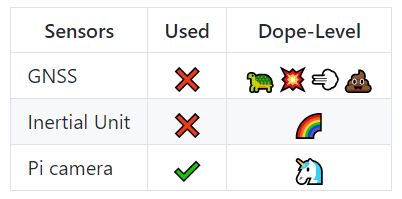
\includegraphics[scale=0.6]{Images/Sensors.png}
    \end{center}
    \caption{The Sensors list available on our GitHub}
    \label{fig:sensors}
\end{figure}

\paragraph{}
As it's shown we decided to choose neither the GNSS nor the Inertial 
Units, mainly because of their accuracy.

\paragraph{}
Actually, for our problem we found that an accuracy of 1 meter
for the \textit{GNSS} is too large because the car need to run in a 0.8 meter
wide racing lane, following a line. This sensors is alos not able to know if
the car position is correct.

\paragraph{}
For the \textit{Inertial Unit}, we found that this sensor is too noisy to
give us any usefull informations about the state of our car. For instance the
consecutive integration of the acceleration in order to get the speed and the
position of the car leads to an important drift effect on our data. So this
sensor is not currently able to to give any correct informations about the state
of the car. Moreover, the acceleration of the car could be quite good after filtering
if we only needed it. In our case the only usefull information is to know the
position of our car in relation to the line.

\paragraph{}
That's why we decided to focus our attention on the camera. Because
we are using a \textit{Raspberry Pi 3B+}, the camera we have choosen is the official 
camera which can be pluged on the dedicated port on the board. This sensor is
perfectly suited to our problem, because with an appropriated image processing
we will be able to detect the line and to correct the car trajectory.

\subsection{Configuration}
\paragraph{}
Now we will explain how we configured our sensors in our project, to
let them comunicate with the software and with the car.

\subsubsection{Pi Camera}
\paragraph{}
The configuration of the camera on the raspberry pi is relatively simple. We
used the \textit{raspi-config} utility to configure the camera. That's how we set up
the camera on the Raspberry Pi.

\begin{figure}[!ht]
    \begin{center}
        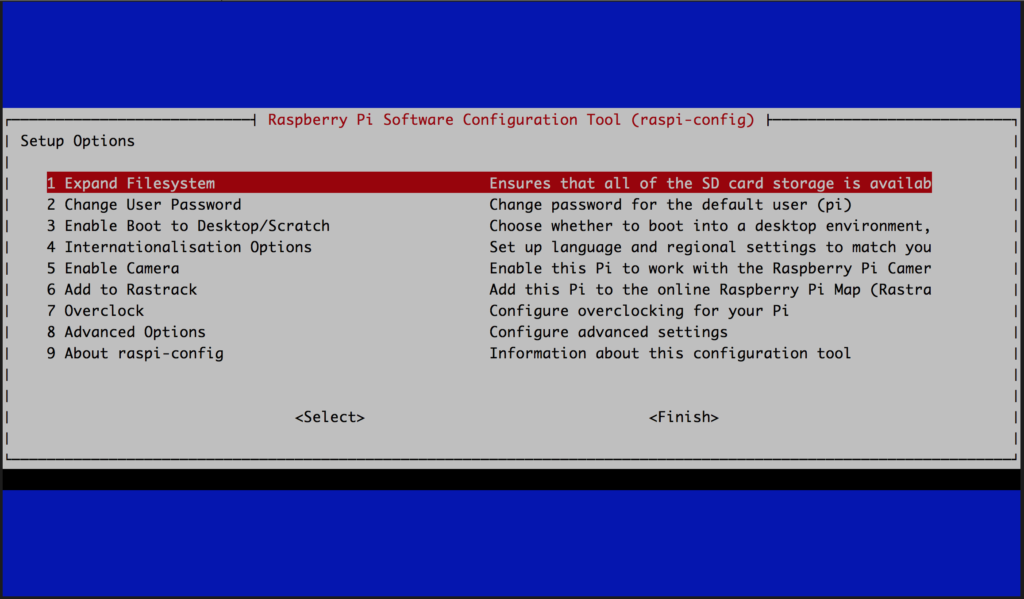
\includegraphics[scale=0.3]{Images/Raspi_config.png}
    \end{center}
    \caption{raspi-config utiliy on the Raspberry Pi}
    \label{fig:raspi_config}
\end{figure}

\subsubsection{Hardware PWM}
\paragraph{}
On Raspberry Pi board there is a lot of way to generate pwm signals.
The most of the time, these methods are software based and so they are not
accurate. With a lot of searches, we found a website who speak about the
raspberry pi's hardware pwm signals. There is apparently an hardware pwm
generator used by the bord to generate sounds. It's better to use hardware 
generated pwm, because if the processor has a slow down and the interrupt
is not correctly handled, the pwm duty cycle will not be very accurate and
the car will not be able for instance to follow a straight line, because the
bearing of the car is controled by a servomotor with a pwm signal.

\paragraph{}So we decided to use this tutorial : \cite{pi_pwm}, 
which explain us how to setup pwm signals on the Raspberry Pi,
and how to correctly configure the files to have a standard pwm signal
which is generated. Then we need to give the rights to users for reading and
writing in these files. All these bash command are in \textit{init\_pwm.sh}.

\paragraph{}
Then we have to add some automation. So we created a \textit{crontab} rule.
That will automatically create all the required files and allow the permissions
to every users. We just have to write in the file \textit{duty\_cycle} a value between
$1.000.000$ and $2.000.000$, and the Raspberry Pi will read and adjust pwm signals
in real time.

\paragraph{}
Last but not least, we setup an autologin in order to open a session automatically
when the Raspberry Pi boot. That's very usefull in order to launch our programms
easily on boot and without any keyboard, mouse or monitor.

\section{Mechanical Architecture}
\subsection{Reasons of an Update}
\paragraph{}
The original architecture of the vehicle was already a good basis for the
realisation of a line tracking car. However, manual manoeuvring tests by
remote control have revealed some driving faults. Defects that could be
disruptive in an autonomous driving mission. Given that our robot
will certainly not be as adaptive as a human in its driving, it is
interesting to ease the maneuvers and correct some mobility deficiencies.

\subsubsection{Problems identified and changes to be expected}
\paragraph{}
Some of the shortcomings noted are listed as follows:
\begin{itemize}
    \item Loss of control due to high front wheel slippage during high speed turns.
    \item In case of sharp turn, locking of the inner wheel on the bend caused by
    the central component box.
    \item Lack of firmness of the front wheel guiding created by a large backlash.
    \item Uncontrolled spinning of the rear wheels when acceleration from a
    standstill or deceleration from high speeds.
\end{itemize}
Since we're starting from the structure of a radio-controlled car not designed to host our computing system (RasPi3, camera, etc.), some components have to be implemented and the structure has to be reworked in order to be an optimal support for autonomous driving such as:
\begin{itemize}
    \item The installation of a camera to see and locate the line to follow.
    \item Hosting a Raspberry Pi 3 card to manage the control computations.
    \item Keep space for the rest of the essential components such as the battery,
    ESC, cables, etc.
\end{itemize}

\subsection{Front Wheel Steering}

\subsubsection{Front wheel slip}
\paragraph{}
One of the major problems that needs to be solved, a problem that could impact
autonomous driving, is the significant slipping of the front wheels when the steering
angle is too large  at high speed.

\paragraph{}
To correct this defect, the best solution would be to improve road handling by
increasing the car's grip. To do this, the wheels would have to be changed from
smooth tires to studded wheels.
However, considering the parts stock available at ENSTA Bretagne, unless we
make an order which would take some time, we did not have better wheels than the
ones proposed.

\subsubsection{Ackermann steering geometry}
\paragraph{}
Nevertheless, we have come up with another solution inspired by normal cars.
The principle of this solution comes from the geometry, especially the steering
geometry of Ackermann.

\begin{figure}[!ht]
    \begin{center}
        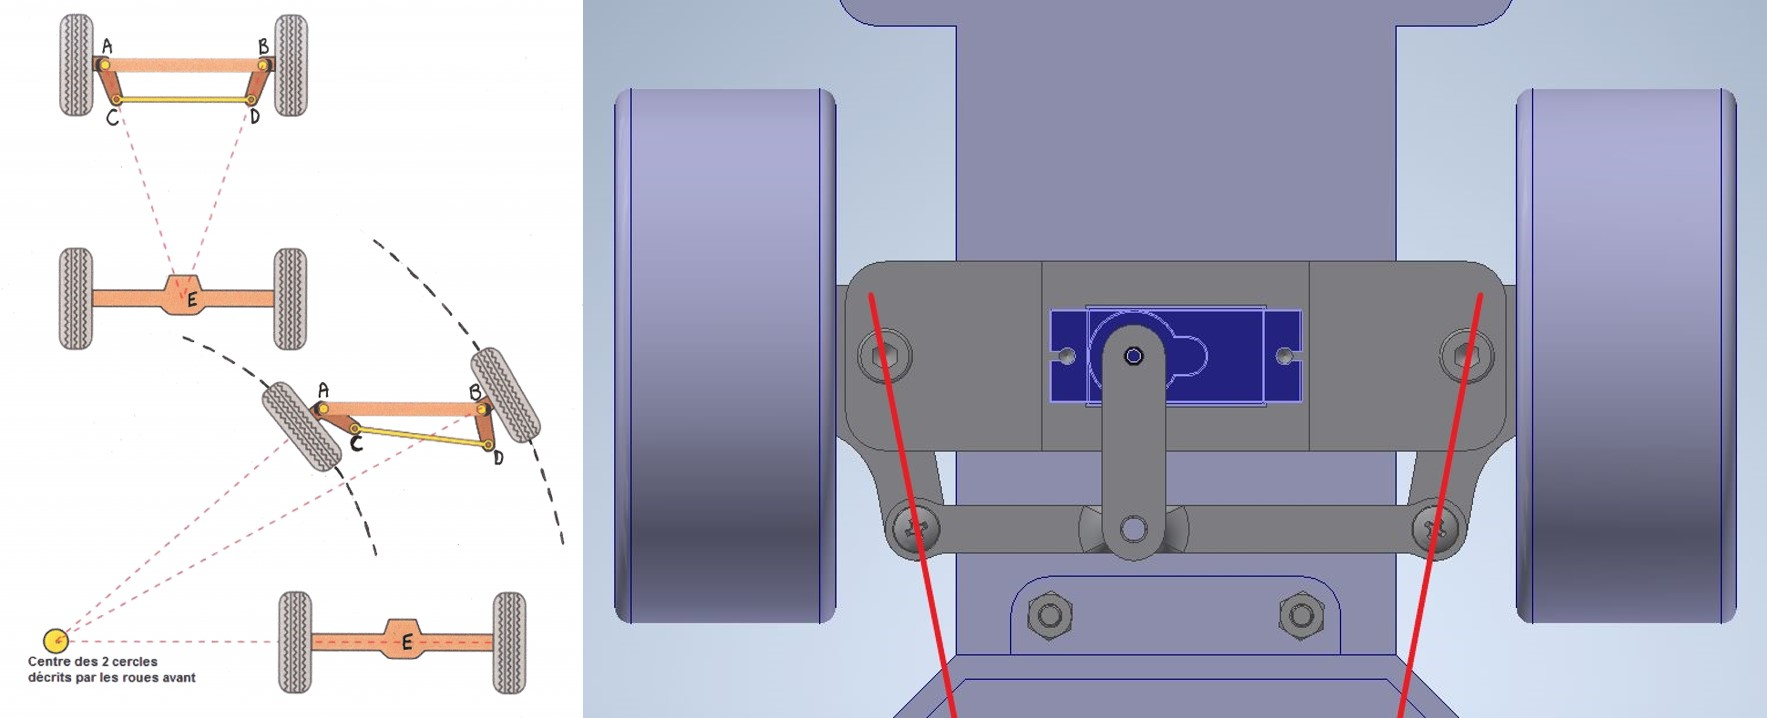
\includegraphics[width=0.9\textwidth]{Images/steering.jpg}
    \end{center}
    \caption{Steering system}
    \label{fig:steering}
\end{figure}

\paragraph{}
The intention is to avoid tyres to slip sideways when following a curved path.
The geometrical solution to this is for all wheels to have their axles arranged
as radii of circles with a common centre point. (See \ref{fig:steering} for more details)
As the rear wheels are fixed, this centre point must be on a line extended from
the rear axle.
Intersecting the axes of the front wheels on this line as well requires that the
inside front wheel to be turned, when steering, through a greater angle than the
outside wheel.

A simple approximation to improve Ackermann steering geometry may be generated by
moving the steering pivot points inward so as to lie on a line drawn between the
steering kingpins and the centre of the rear axle.

\paragraph{}
We have therefore redesigned the pivot points to respect this geometry. We also
took advantage of this to improve the bearing embedding system that connects the
bearing to the wheel so that the steering wheels are held more firmly.

\subsection{Front Camera Support}

\subsubsection{Camera support structure}
\paragraph{}
We then had to implement the camera that would allow our robot car to have eyes
on the road.

In order to position it correctly, the camera had to be able to stand back enough
on the road in front of it and the angle of view had to be horizontal enough to see
far away but with a high enough incidence to identify the line without being
hindered by the sun's reflections on the road. This results in false identification
of the lines and then adds errors in the guidance.

\begin{figure}[!ht]
    \begin{center}
        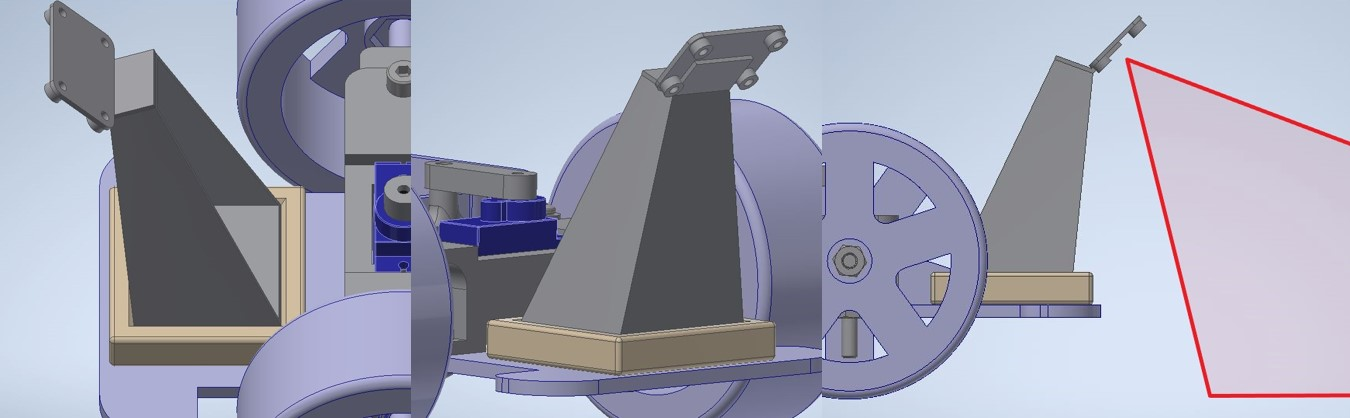
\includegraphics[width=0.9\textwidth]{Images/camera_support.jpg}
    \end{center}
    \caption{Front camera support structure}
    \label{fig:camera_support}
\end{figure}

We have therefore designed a structure that raises the camera a few centimetres
above the chassis and tilts it at 45 degrees towards the ground. 

\subsubsection{Vibrations issue}
\paragraph{}
Our car will be driven in a natural environment and the ground will probably
be slightly bumpy and gravelly. The chassis will be
subjected to many vibrations and at the same time, the camera may be subject to
vibrations transmitted by the chassis. These can degrade the performance of the
image processing algorithms.

\paragraph{}
One of the simple mechanical solutions to reduce these disturbances is to dampen
the vibrations in the connection between the chassis and the camera by using for
example a silentblock.
We used a soft synthetic foam as a silentblock to counteract these vibrations.
(See \ref{fig:camera_support} for more details)

\subsection{Component Hosting Box}

\subsubsection{Additional space}
\paragraph{}
In order to host the necessary additional electronics we needed to increase the
space to host the components. We redesigned the box by increasing its width.
In its new dimensions, the box offers twice as much space without unbalancing
the overall structure.

\begin{figure}[!ht]
    \begin{center}
        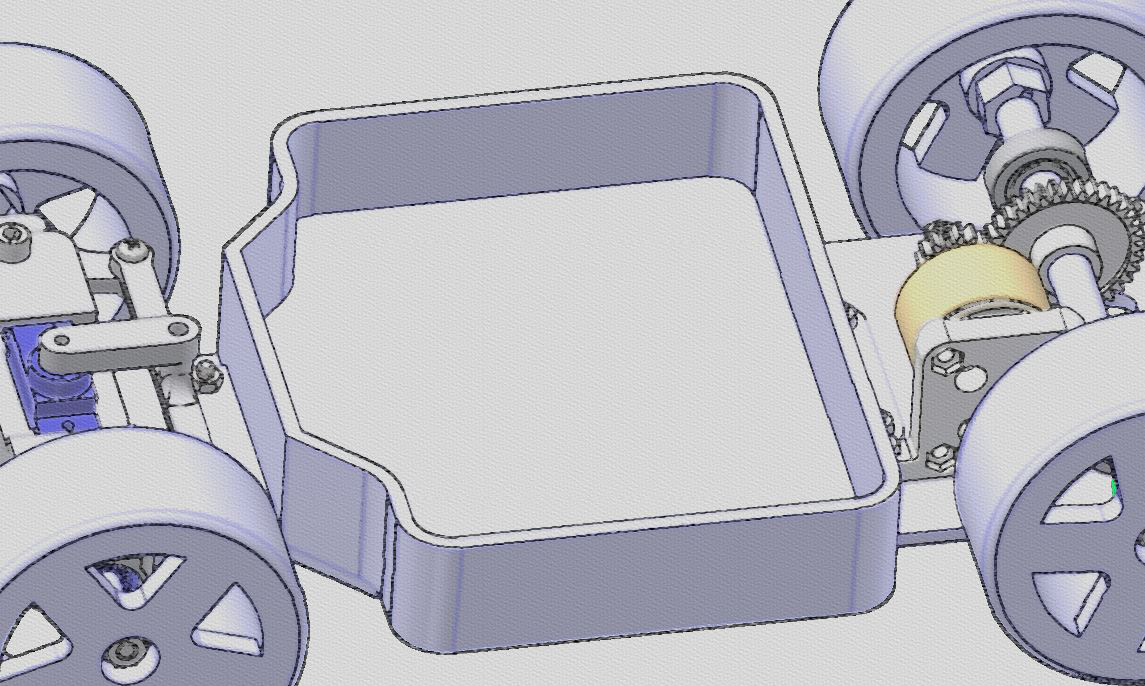
\includegraphics[width=0.9\textwidth]{Images/kart_central_box.png}
    \end{center}
    \caption{Central component box}
    \label{fig:central_box}
\end{figure}

\subsubsection{Carved box}
\paragraph{}

In the process of creating a new box, we took the opportunity to correct one
of the problems caused by the front corners that blocked the steering wheels
when they were fully steered. So we took the care to add two notches in
the place of these corners to allow the wheels to move without hitting them.
(See \ref{fig:central_box} for more details)

\subsection{Expectations and Reality}
\paragraph{}
As you may probably know, there is a difference between expectations and the
actual reality.

\paragraph{}
The plans were good, but an unprecedented event came to modify them, as a
consequence of the proliferation of covid-2019, the school had to close its
doors. Deprived of manufacturing means and having only one prototype for the
group, we had to stick to what was already done. With DIY, hot glue and a
bit of common sense we were able to come up with a modest but acceptable
structure.

\paragraph{}
Although the final structure of our car does not have all the improvement
imagined, it still in acceptable condition for autonomous driving in an
environment like a traditional athletics track.

\begin{figure}[!ht]
    \begin{center}
        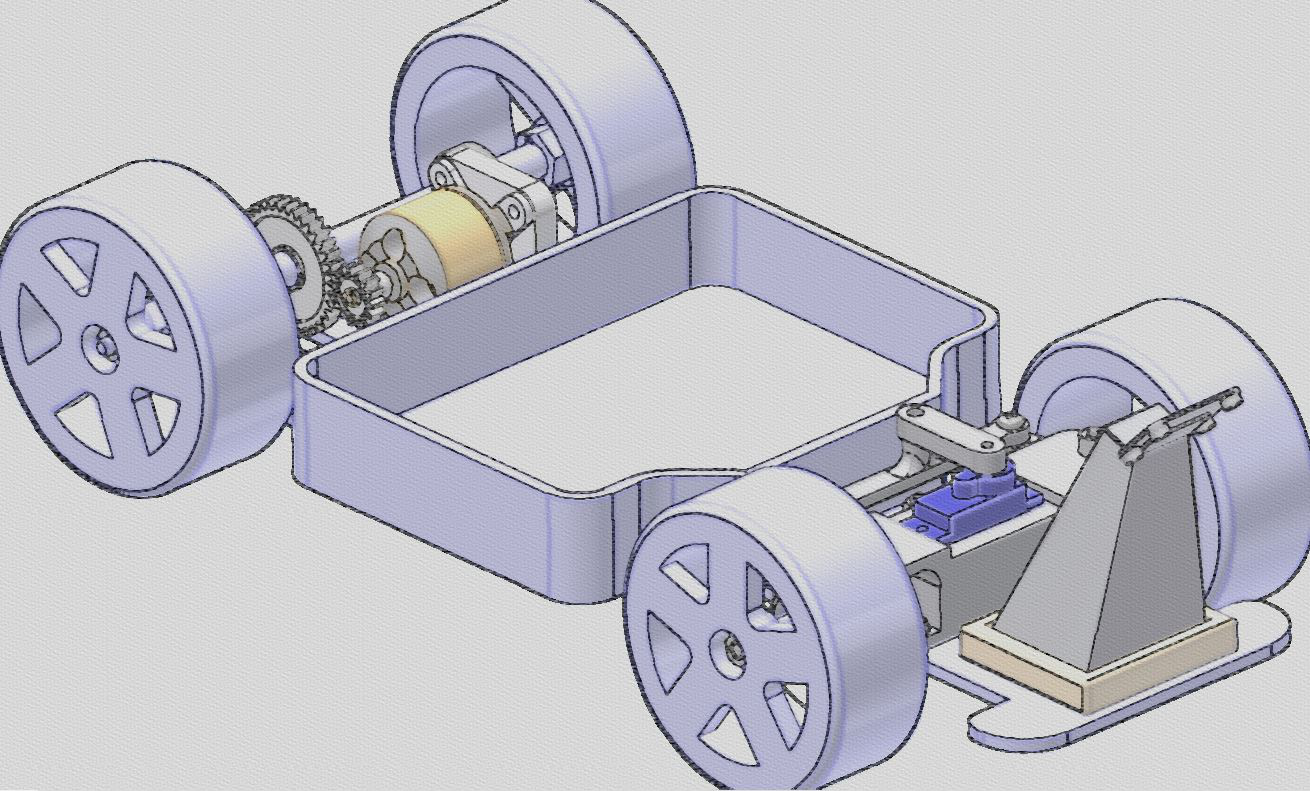
\includegraphics[width=0.9\textwidth]{Images/plan_global.png}
        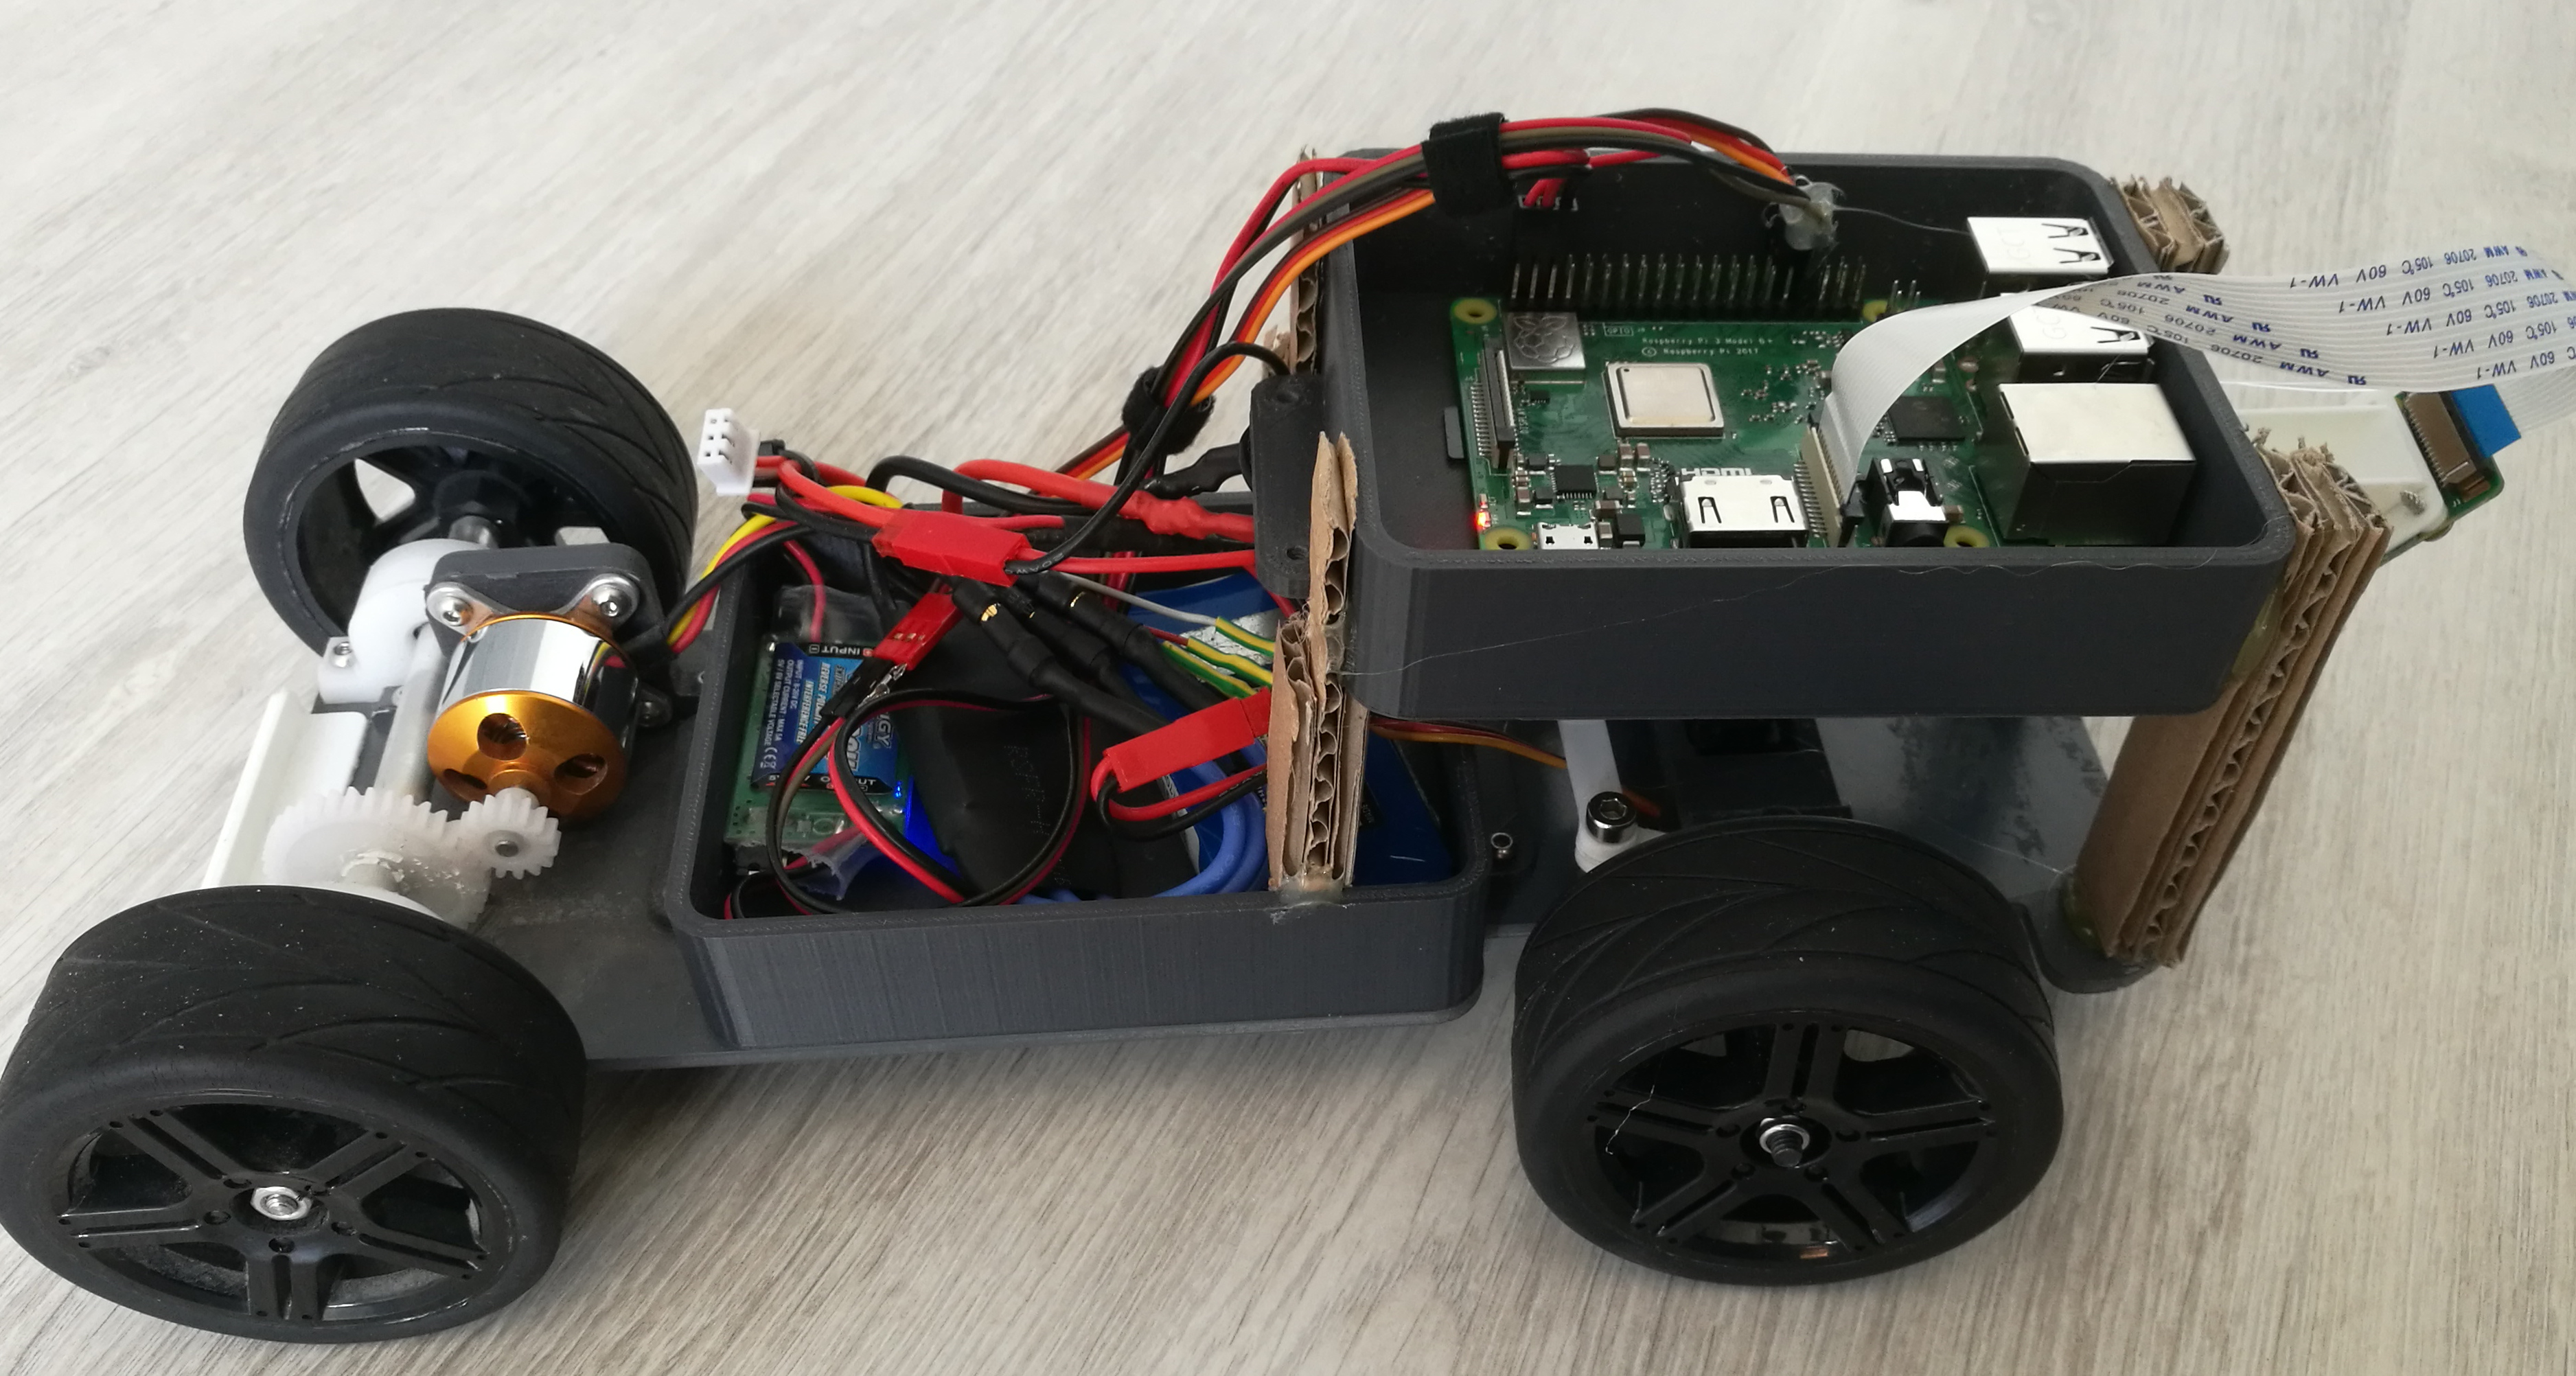
\includegraphics[width=0.9\textwidth]{Images/Kart_overview_1.jpg}
    \end{center}
    \caption{Expextations and reality}
    \label{fig:expectation_reality}
\end{figure}

\paragraph{}
In the final model, the proposed solutions include Ackermann's steering
system and the system for embedding the bearings connected to the steering
wheels. The front camera support had to be totally modified but the intentions
are the same even though there is no damping system. And the housing box has
remained the same but has been doubled on a second floor to contain the
electronic components.
By limiting the rotational movement of the steering wheels, we can ensure
that the front wheels do not get stuck.
(See \ref{fig:expectation_reality} for more details)

Although the final structure of our car does not have all the improvement
imagined, it is still in acceptable condition for autonomous driving in an
environment like a traditional athletics track.


\section{Image Processing}



\paragraph{}
To carry out the image processing we used very simple theoretical notions. The library we used is open cv. The figure below summarizes our image processing.
\begin{figure}[ht!]
    \begin{center}
        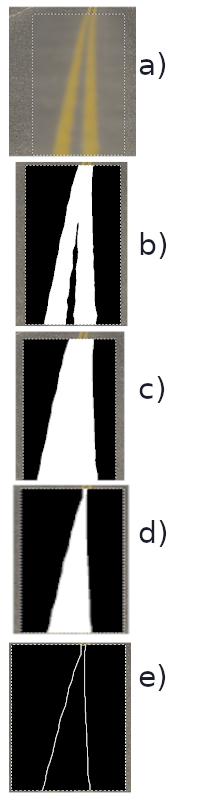
\includegraphics[scale=0.3]{Images/diagramme.png}
    \end{center}
    \caption{image processed}
    \label{fig:img_processing}
\end{figure}

\subsection{Data logging}
\paragraph{}
For the first part of this image processing, we had to collect images.
So first we went into the environment in which the robot was going to evolve.

\begin{figure}[ht!]
    \begin{center}
        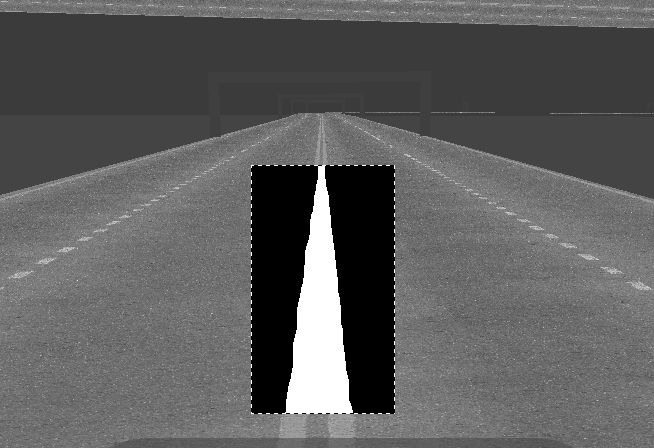
\includegraphics[scale=0.3]{Images/image_process.png}
    \end{center}
    \caption{image processed}
    \label{fig:img_processing}
\end{figure}

\subsection{pre binarization treatment}
\paragraph{}
In this part, we first had to perform a pre-binarization treatment in order to reduce post-binarization noise.
So we used a Gaussian filter to blur the image.

\subsection{binarization}
\paragraph{}
Since the line we wanted to mark is white. An effective treatment is simply to switch to grey level. 
So for binarization, we switch the image to a grey level and threshold for a grey level that we have determined empirically.

\subsection{post binarization treatment}
\paragraph{}
In this part we performed a morphological treatment. There was still a lot of noise after binarization. So we made an opening. 
With a kernel in the shape of a rectangle (since it was the most efficient for this treatment).
At the end of this treatment we obtain a well defined line which crosses the screen.

\subsection{find the center of the line}
\paragraph{}
In this last part, the contours are marked using a gradient method. Then the contours are sorted from the smallest to the largest.
We recover the largest contour.
And we recover the coordinates of the barycentre of the contour.
Then the error is the difference between the center of the image and the coordinates of the pixel.
The problem with this method is that with the barycentre we have a regulation on a point in the centre of the image. And therefore, we don't use all the data we have.
So we decided to use the highest points of the contour.
Indeed, the position of the center of the line at the highest point of the image gives us an idea of the evolution of the road at the moment. From now on we use the horizon. It allows us to get information further into the "future". And so it allows for better regulation and therefore to go faster.


\section{VREP Simulation}
\subsection{Explaination}

Based on the practical work made with Benoit Zerr, we made a realistic track with a line in the middle \cite{zerr}.
The simulated in VREP car is equiped with a camera. Our VREP simulator is interfaced with ROS through the piece of LUA code :

\begin{figure}[ht!]
    \begin{center}
        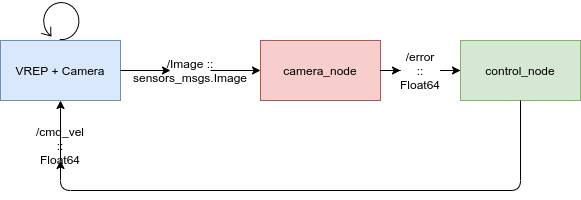
\includegraphics[scale=0.5]{Images/graph_node_simulation.png}
    \end{center}
    \caption{Graph node of the simulation}
    \label{fig:graph_node_simulation}

\end{figure}

As it is explained on the figure \ref{fig:graph_node_simulation}. The VREP camera send a through a topic \texttt{image}, a picture of the front of the car. 
Then the \texttt{camera\_node} subscriber process the image with OpenCV and return the position
of the barycenter of the line (red in the figure \ref{fig:command_explanation}), then it compute an error, we want the barycenter of line in the middle of the windows, as it's shown on figure \ref{fig:command_explanation}. 
This error is sent through a topic \texttt{error}, the controller is suscribed to this topic,
it generate a command thanks to a PD command law which is sent to VREP. And now the car can loop forever, and achieve 
the perfect run in 1'15'' !

\subsection{Regulation}
\begin{figure}[ht!]
    \begin{center}
        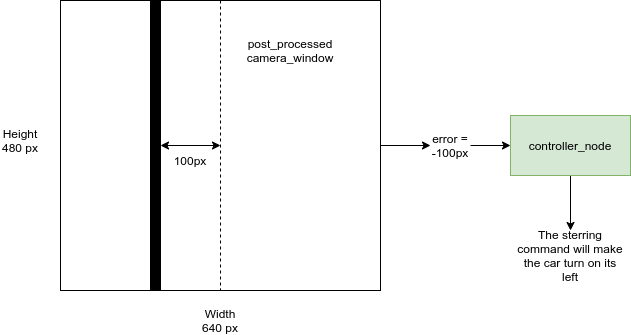
\includegraphics[scale=0.5]{Images/command_explanation.png}
    \end{center}
    \caption{Explanation of the command : line in black, barycenter in red}
    \label{fig:command_explanation}

\end{figure}
We implemented a PD regulation. Let's call $(c_x, (c_y)$, the barycenter of white line, the car is required to stay in the middle of the line.
Therefor we compute an error : $e = (width/2 - c_x) + (height/2 - c_y)$ and then the command u equals : 
$u = K_p e + K_d \frac{de}{dt}$. This command is computed in the controller and sent to vrep.


The result in video : \footnote{\url{https://www.youtube.com/watch?time_continue=10&v=_vIXo1TvG0w&feature=emb_logo}}  






\section{Localization}
\subsection{Problem in Localization}

\paragraph{}
In this project, we decided to realize the challenge through visual servoing.
That is to say a line tracking by the camera. This type of servoing only
works if the robot has at all times the line to follow in its field of vision. 
But this is not possible since it will very often happen that the robot loses sight of the line. Especially during a turn. So if our car loses sight of the line, we'll have to get it back on the track.


\paragraph{}

\subsection{Robot status estimation}

\paragraph{}
To compensate for this very likely situation, 
we have a control law in place that will be used as soon as the robot loses the line. 
This law of control requires knowledge of the robot's condition.

\begin{figure}[!ht]
    \begin{center}
        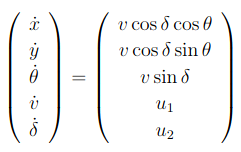
\includegraphics[scale=0.6]{Images/Etat_tricycle.png}
    \end{center}
    \caption{State of the robot}
    \label{fig:State}
\end{figure}

\paragraph{}
Where (x,y) is the position of the robot, $\theta$ is its heading, v its speed and $\delta$ the angle of the front wheels.
To be able to apply a Kalman filter we need a linear state representation of the robot. To make these equations linear, 
we have considered the angle $\theta$ of the robot as an input (since it is given by the inertial unit). 
This removes equation 3. Then we linearized the equation into xhat (xhat being the new state to be determined).xhat consists of x,y, $\theta$, $\delta$. 
The file  available on our github shows the function of this Kalman filter.


\begin{figure}[!ht]
    \begin{center}
        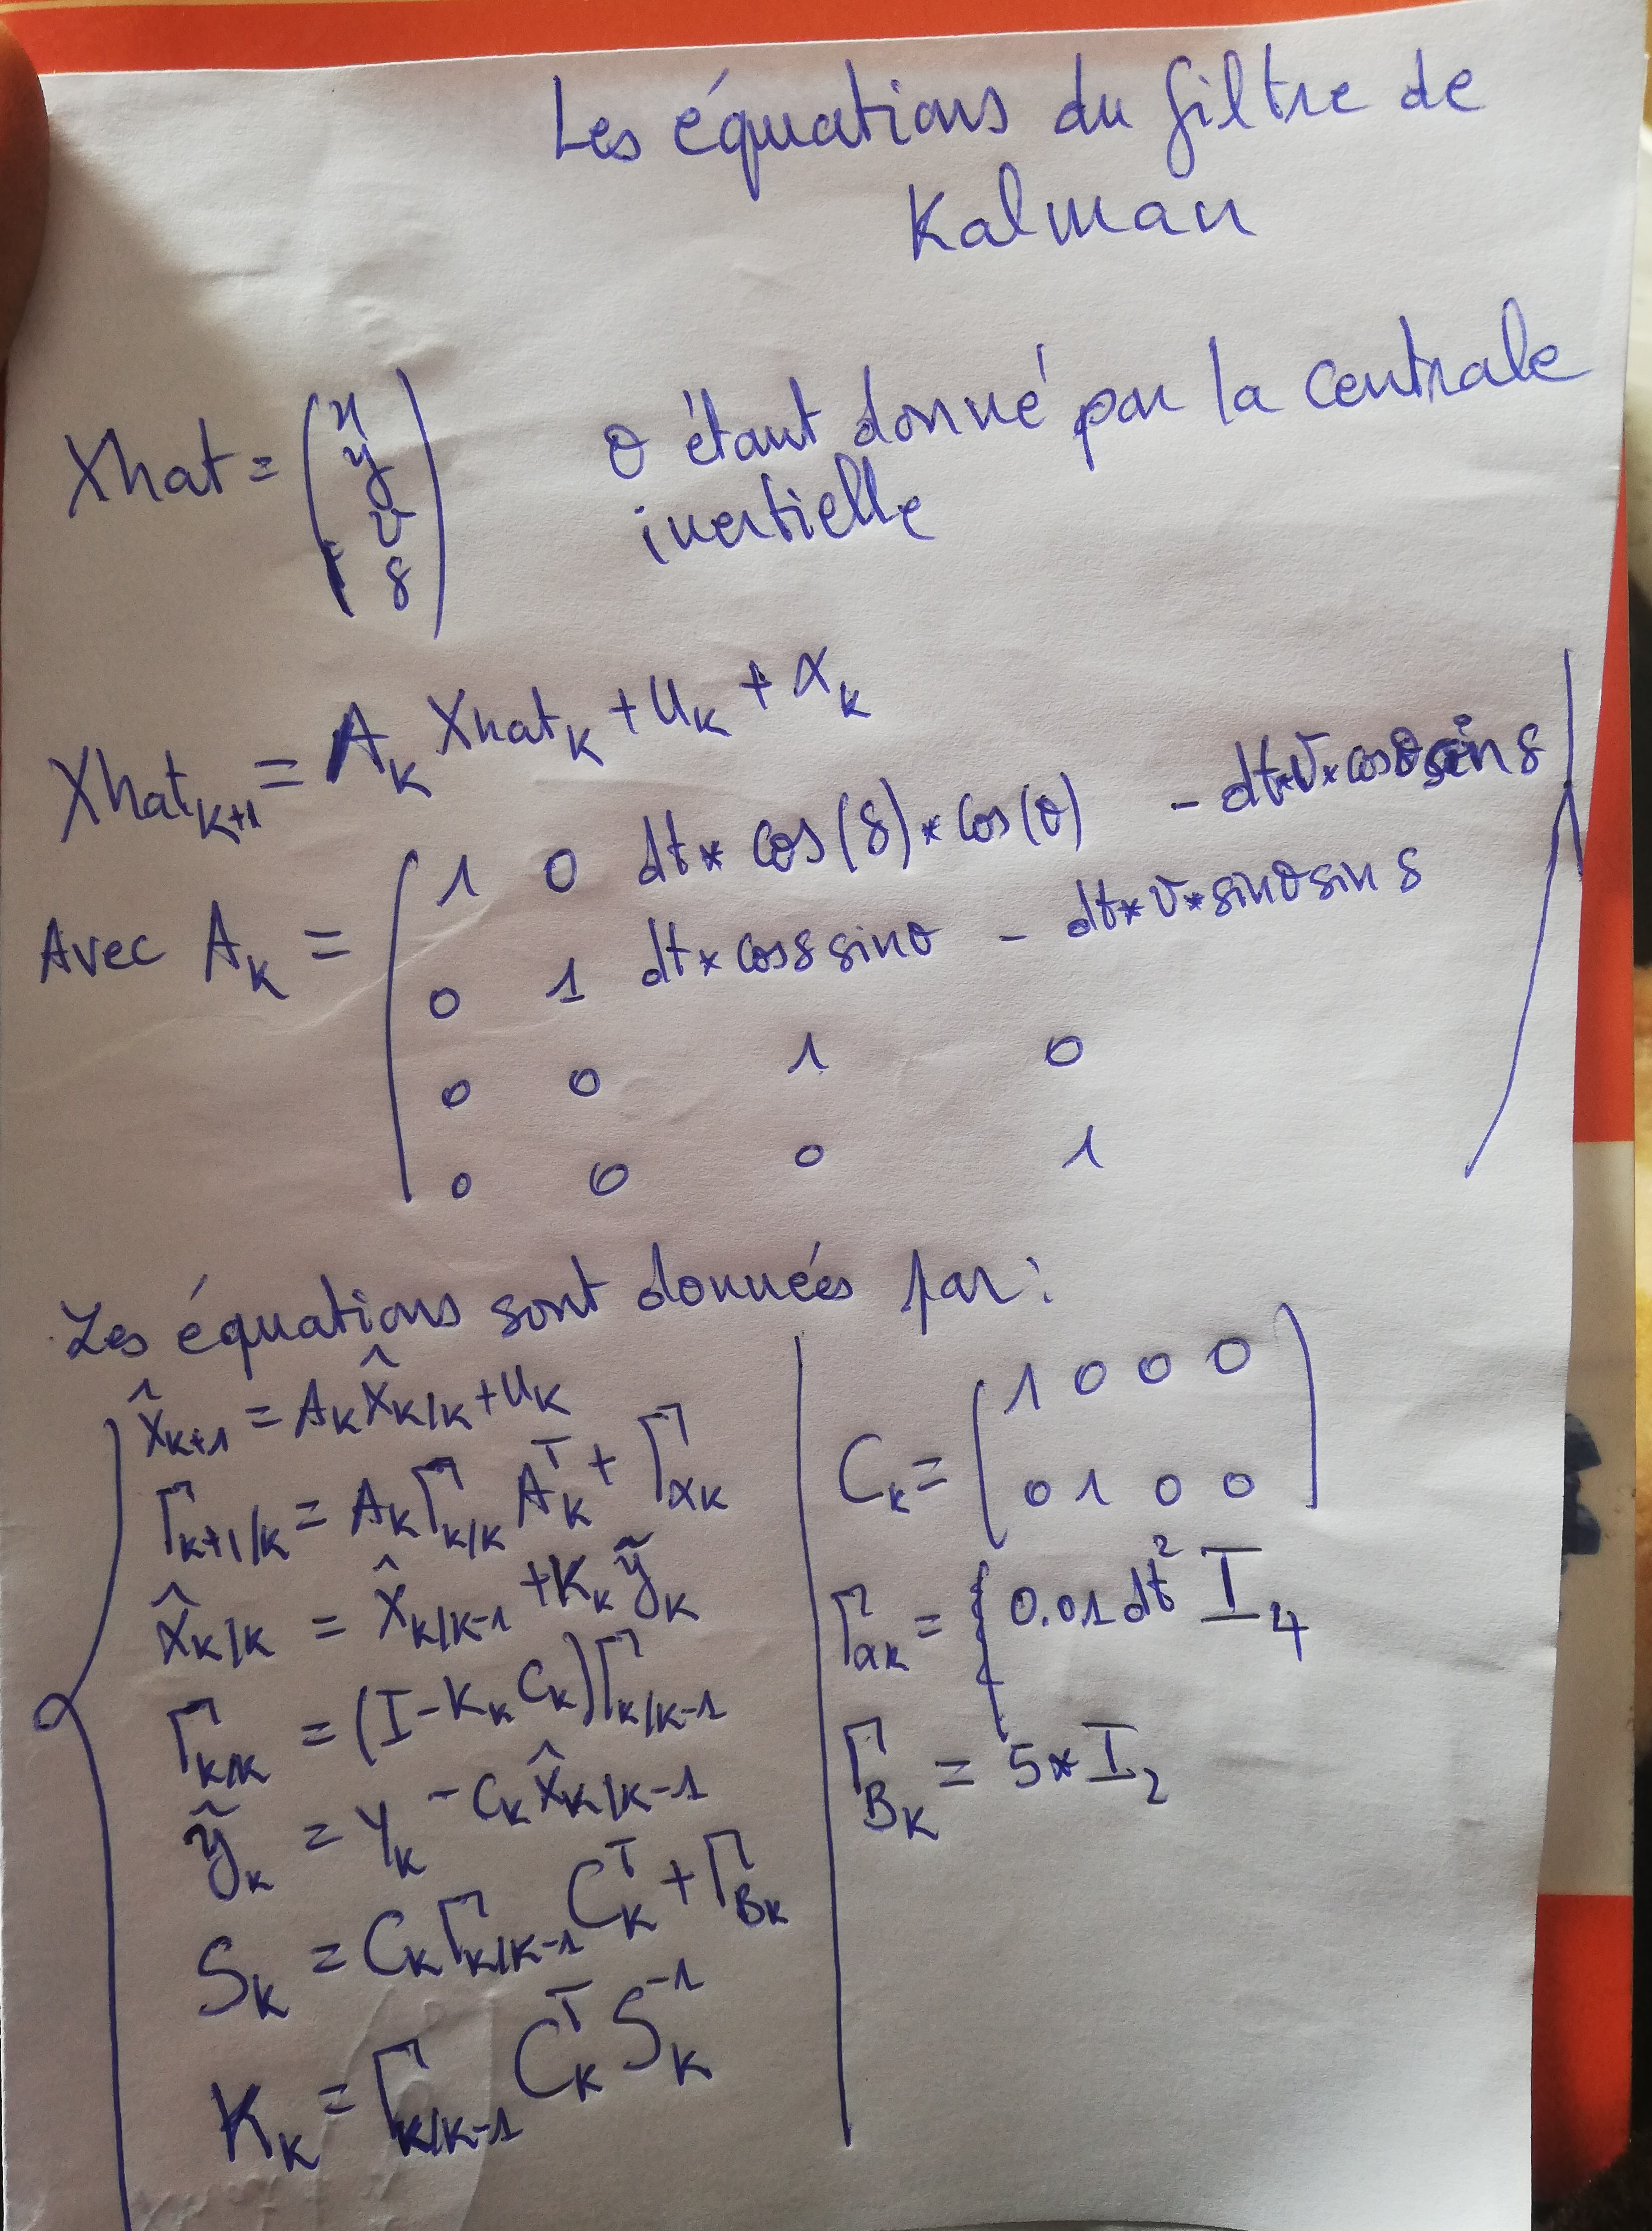
\includegraphics[width=\textwidth]{Images/Equation_filtre_K.jpg}
    \end{center}
    \caption{Kalman Filter Equation}
    \label{fig:Equation}
\end{figure}




\section{Explications}



\section{Resultats}
\input{Chapters/04_Results}


\section{Discussions et Conclusion}
To conclude, we think that we already have a strong basis for this project, particularly
with the ROS structure  which is already setup. Then we have to perform test with the
real system because the simulation is correctly working and a good proof of concept, 
but we lnow too that simulation and reality are always different. We have to do some
improvements on our projetc too, like adding an mission controler in order to control the
robot in some cases where we couldn't use the line following command, for instance when the 
camera is not seeing any lines, and we ha to add a GUI in order to show the kart state
like his position, is speed and the circuit.

\section{Improvements}
\subsection{Prerequisites}
This part will be implemented in the future and are for now only some good
ideas we have for this project. We are first focused on the achievement of the simple
control of this car.

\subsection{Mission}
We have establish a simple command for our kart based on image processing. This
command law is quite easy to setup and fully functionnal as we could see. However
this command is efficient only if the camera is able to see a line. But actually
the car could be unable to see a line, particularly when the car will accelerate
in order to run a lap as quick as possible. Our strategy on this topic is to run
a first lap very slow and to drop virtual gps tags on a map while the car is following
the line. So after a lap we will get a whole map of the circuit and at any given times
the car will have to determine if a line is available on the camera, and if the car
could follow this line, else the car will have to reach this line again with the help
of the gps tags. Then after the first lap, the car will be able to accelerate and for instance some times
lost the line because it will be able to reach again the circuit with the gps tags.

\subsection{GUI}
We found quit interresting to have a beautifull Graphical User Interface for our
car. We are thinking about a frontend solution in order to show dynamical parameters
such as acceleration and seep of the car, and a map to show the position with the 
classical circle to represent the incertainty of this position. Moreover it could
be interresting to have the camera output available on this GUI. The easiest way to
display a map and some gnss coordinates on python is to use the \textit{folium} package
based on the \textit{OpenStreetMap} map. We are now working on a bind between \textit{ROS},
\textit{folium} and the web framework \textit{Django} to sum up these informations on
a state webpage. However, we don't own any GNSS or Inertial Units to prepare hardware
nodes. That is also not our prioriy, but it can be a very usefull tool.



%\bibliographystyle{plain}
%\bibliography{Bibliography.bib}

\appendix
\section{Appendix}
\input{Chapters/06_Appendix1}


%---------------------------------------------------------------------------------
%	Example SECTION (Remove this section to finalize the report.

% Remove this line to finalize the report.
%---------------------------------------------------------------------------------


\end{document}


% Note: Again, you don’t need to answer just the above questions. They are being provided to give you a flavor of what is required for each section. Use your judgment and initiative to add or subtract based on the specific homework. You can add any other conclusion or discuss any other aspect of your effort that you think it is important to highlight.

% Also ensure to attach the MATLAB or MULTISIM files with this report
